\chapter{Introduction}
\label{ch-introduction}

The aim of the work that is presented in this thesis is to make a contribution improving grid operation and reliance when using Battery Energy Storage Systems (BESS) in the UK Low-Voltage (LV) power distribution networks by adjusting sub-half-hourly operation and communication regimes of the BESS.
In this context, grid operation performance is considering mainly peak power flow, but also includes voltage deviation, phase imbalance, distribution losses, and the magnitude of neutral currents.

Provide grid support is expected to become a vital necessity since the predicted increase in electricity demand and demand volatility will negatively effect the performance of the UK distribution networks.
Due to the network's design and topology higher and more volatile demand is predicted to cause issues including voltage deviation, asset overloads, equipment damage and, in the worst case, service disruptions.
As discussed in this thesis, BESS is a suitable alternative to traditional network reinforcements, however, successfully combining fast system response capabilities (i.e. at sub-half-hourly resolution) with traditional operation schedules (i.e. at half-hourly resolution) to yield the best impact on network performance (e.g. peak-reduction) is still an open research question.
Also, with the proliferation of household-connected BESS and Electric Vehicles (EVs), performance of algorithms that coordinate their operation are also an ongoing research topic.

In this chapter, Chapter~\ref{ch-introduction}, the background and motivation for the conducted research are presented.
Then, on the basis of the identified challenges and opportunities for battery energy storage in the electricity distribution network, the problem statement and all research objectives are outlined.
At the end of this chapter, all contributions and publications are stated, and the structure of the rest of this thesis is presented.

\section{Background and motivation}
\label{ch-introduction:sec:background}

% - Background
%   - Electricity grid
%   - Role of energy storage - a survey

Today's society and economy are highly dependent on the continuous availability of energy, or more specifically: electric energy.
Demand for electricity has increased over the past decades, and this trend is expected to continue into the future \cite{HMGovernment2009}.
This demand increase is only accelerated since major focus of UK energy policies has been put on transitioning towards a low carbon economy \cite{RoyalAcademyofEngineering2010}.
Particularly the decarbonisation of heat and transport sectors are two areas of significant strategic focus and Low Carbon Technology (LCT) such as Photo-Voltaic (PV) installations, electric vehicles and heat pumps are expected to contribute significantly to this transition.

However, as adaptation of these LCTs increases and they start to penetrate power distribution networks, stress on these networks will continue to increase even further, which may result in additional service disruptions.
Furthermore, the uptake of LCTs is not expected to progress evenly throughout the entire power network, and instead clusters of early adopters are predicted to form, leading to certain Low-Voltage (LV) networks to exceed their operational constraints even at relatively low national rate of LCT adaption \cite{Poghosyan2014}.
The scale of this energy transition becomes becomes particularly apparent when referring to the UK's future energy scenarios that compare the predicted future load scenarios.

\begin{figure}\centering
	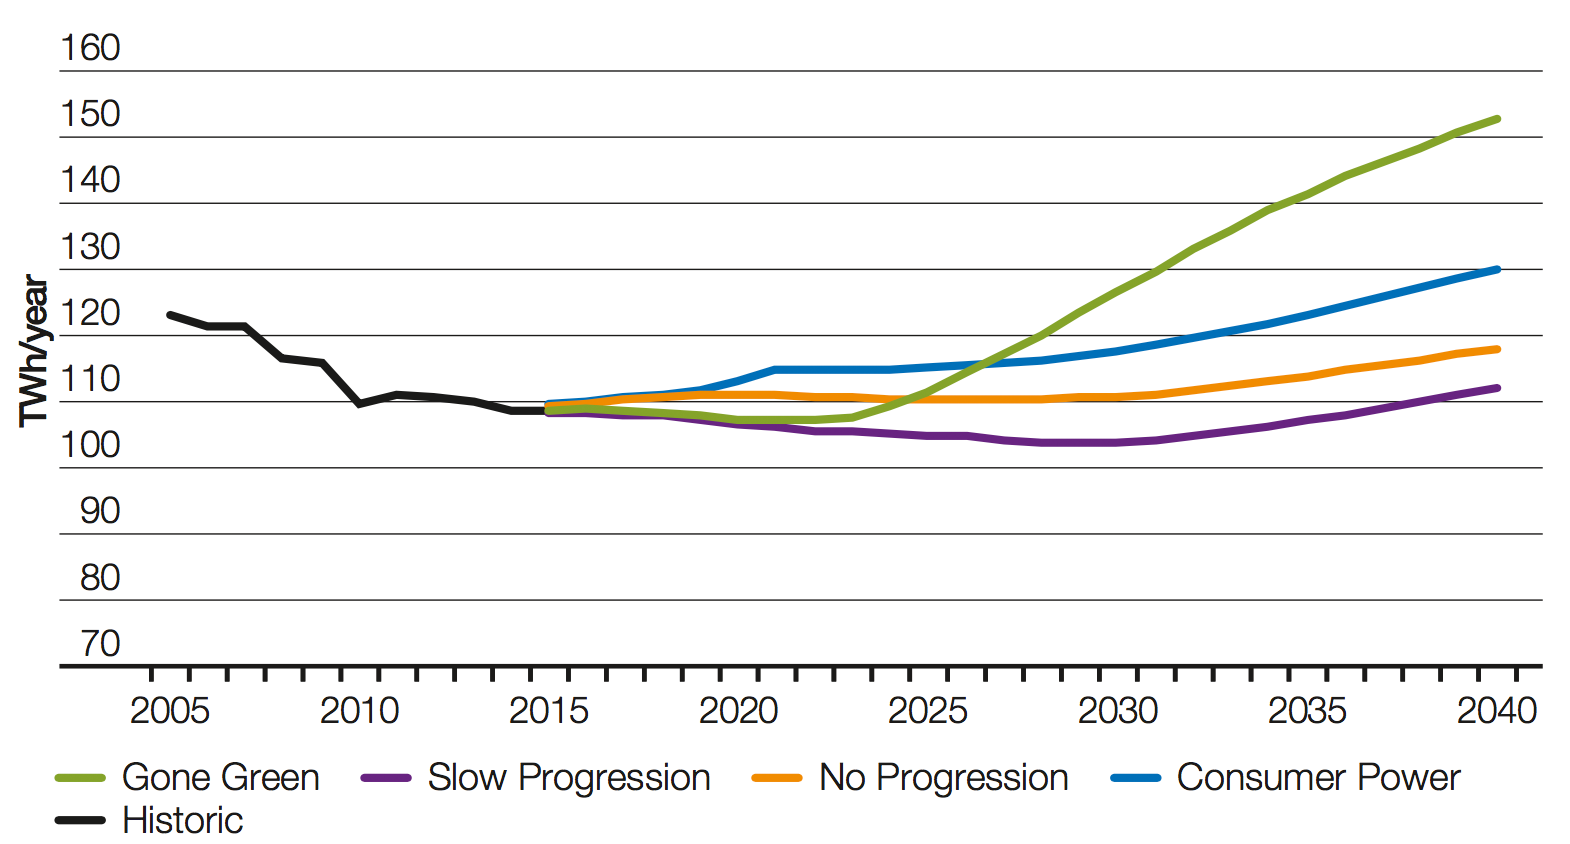
\includegraphics{_introduction/fig/electricity-demand-forecast}
	\caption{Annual residential demand for electricity from FES2016 \cite{FES2016}}
	\label{ch-introduction:fig:electricity-demand-forecast}
\end{figure}

Figure \ref{ch-introduction:fig:electricity-demand-forecast} shows the predicted increase in demand for electric energy when following the UK's 2020 and 2050 goals in reducing green-house emissions.
According to this projection, the annual energy demand will increase by more than 40TWh by the year 2040, if the ``Gone Green'' approach is implemented.
This trend is expected despite increasing device efficiencies, since the shift from oil and gas to electricity, i.e. the electrification, offset these gains.

\begin{figure}\centering
	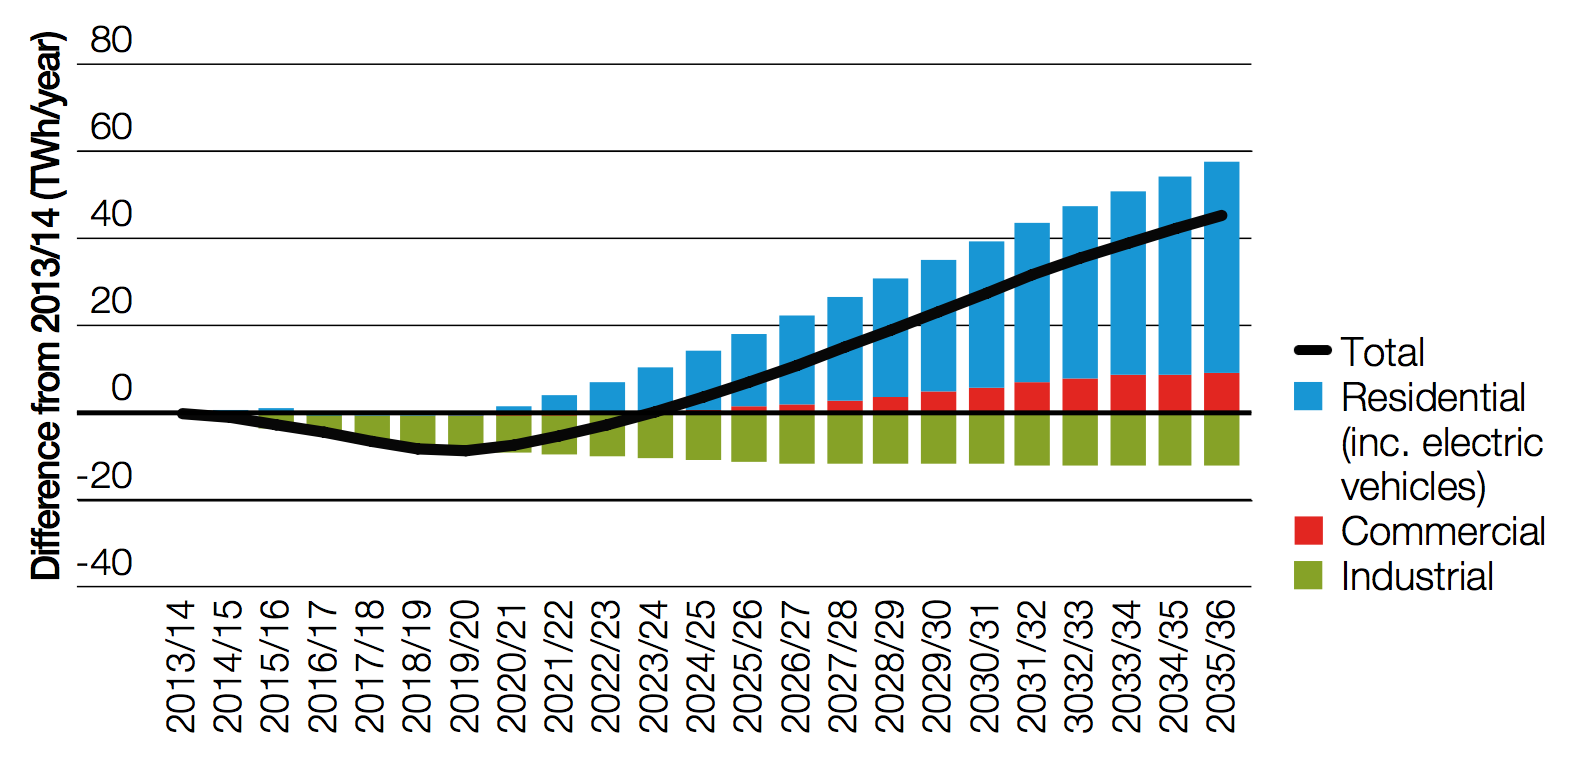
\includegraphics{_introduction/fig/electricity-demand-change-forecast}
	\caption{``Gone Green'' power demand comparison to 2013/14 by type (excluding losses) from FES2015 \cite{FES2015}}
	\label{ch-introduction:fig:electricity-demand-change-forecast}
\end{figure}

\nomenclature[G]{CREST}{Centre for Renewable Energy Systems Technology}

When breaking down the change in demand for electricity, as done in Figure \ref{ch-introduction:fig:electricity-demand-change-forecast}, one can observe how industry sectors are expected to decrease their energy consumption.
Yet residential and commercial sectors are expected to increase their demand and outweigh the industry's energy savings.
Their negative impact on the distribution network is only amplified, since loads in the residential and commercial sectors are typically situated at the network edge, i.e. in the LV distribution network.
This part of the network is its weakest part, since its assets were designed to caters for small powers between 315kVA to 500kVA \cite{EDS08-0115}.
A study based on the findings from \textit{Electricity North West} in \cite{ElectricityNorthWestLtd2014} emphasises the issues that result from residential increase in demand for electricity, of e.g. voltage deviation due to an uptake of LCTs.
The voltage deviation and corresponding power profiles are shown in Figure \ref{ch-introduction:fig:lct-impact}, which was produced by simulating several loads on the IEEE LV Test Case power distribution feeder.
Loads were modelled at high resolution, using the \textit{Centre for Renewable Energy Systems Technology} (CREST) dwelling model \cite{Richardson2010a} and a subset of loads was adjusted using a normal and Rayleigh distribution for solar irradiance and home-charging EVs, respectively.
The findings in Figure \ref{ch-introduction:fig:lct-impact} show how uncontrolled home-charging of EVs significantly reduces voltages in the network, and although solar injection does lead to voltage rises along the feeder, unbalanced injection increases voltage deviation even further.

\begin{figure}\centering
	\subfloat[]{
		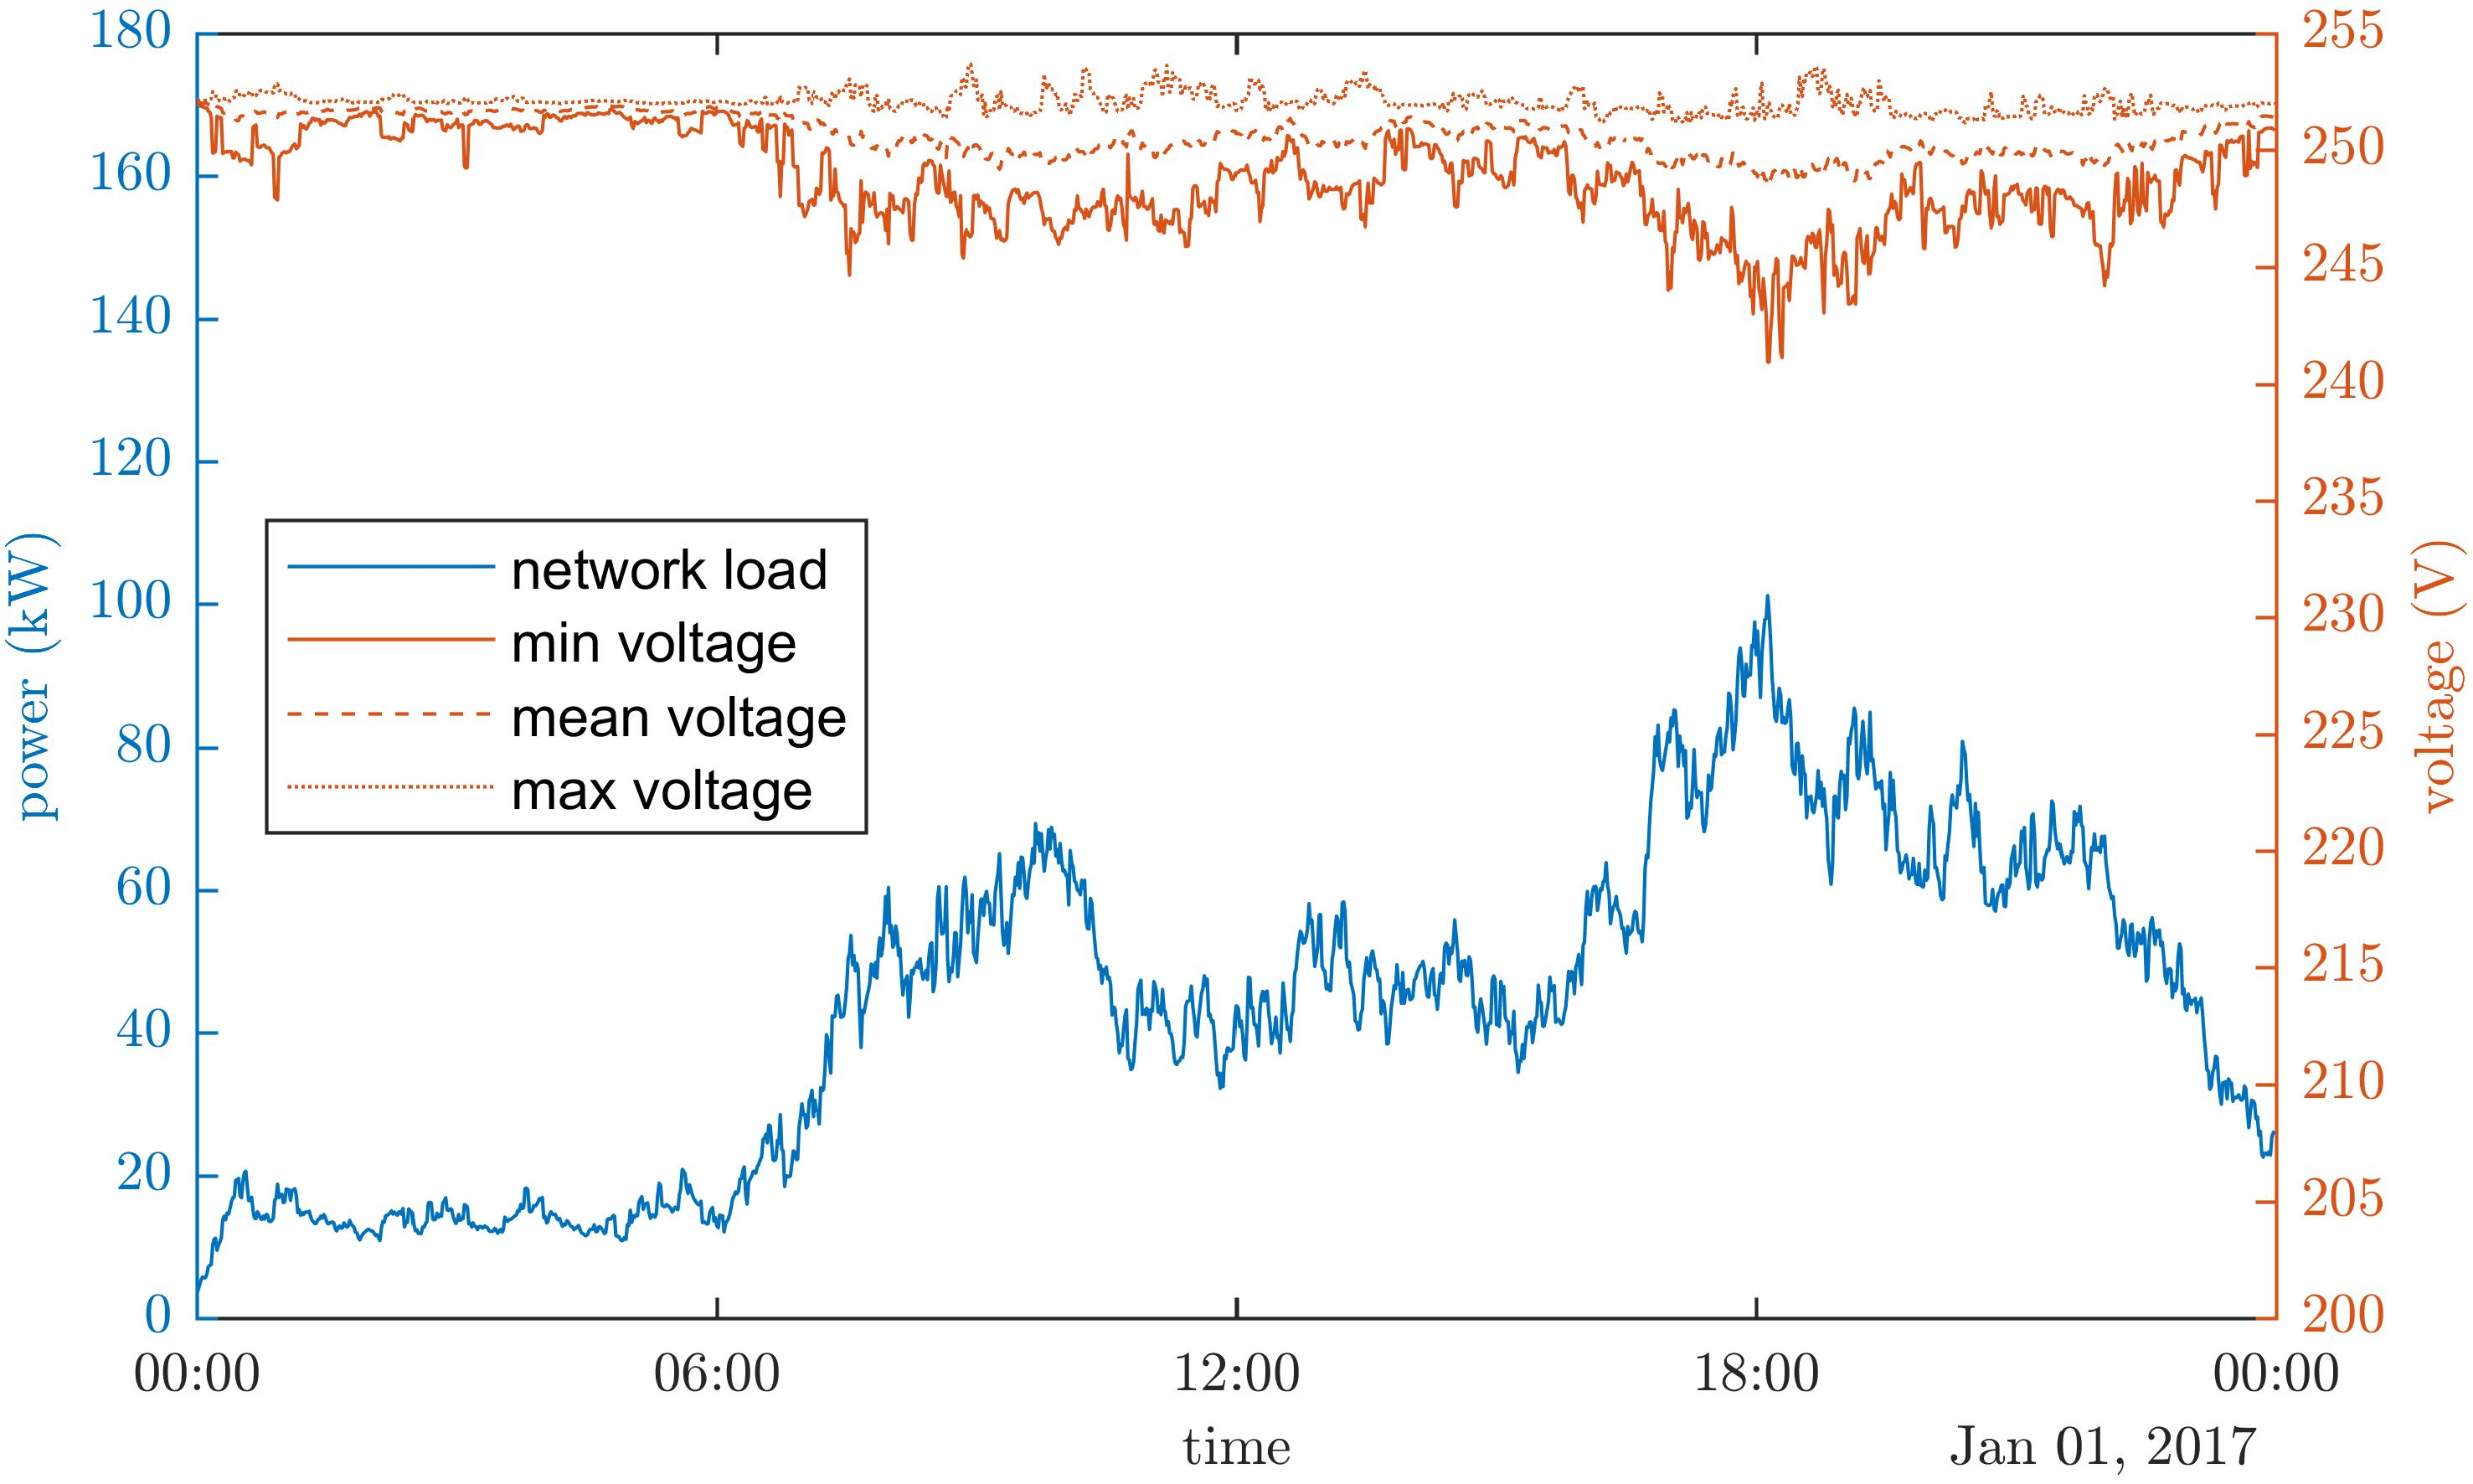
\includegraphics{_introduction/fig/lct-impact-without}
		\label{ch-introduction:subfig:lct-impact-without}
	}
	\vspace{1mm}
	\subfloat[]{
		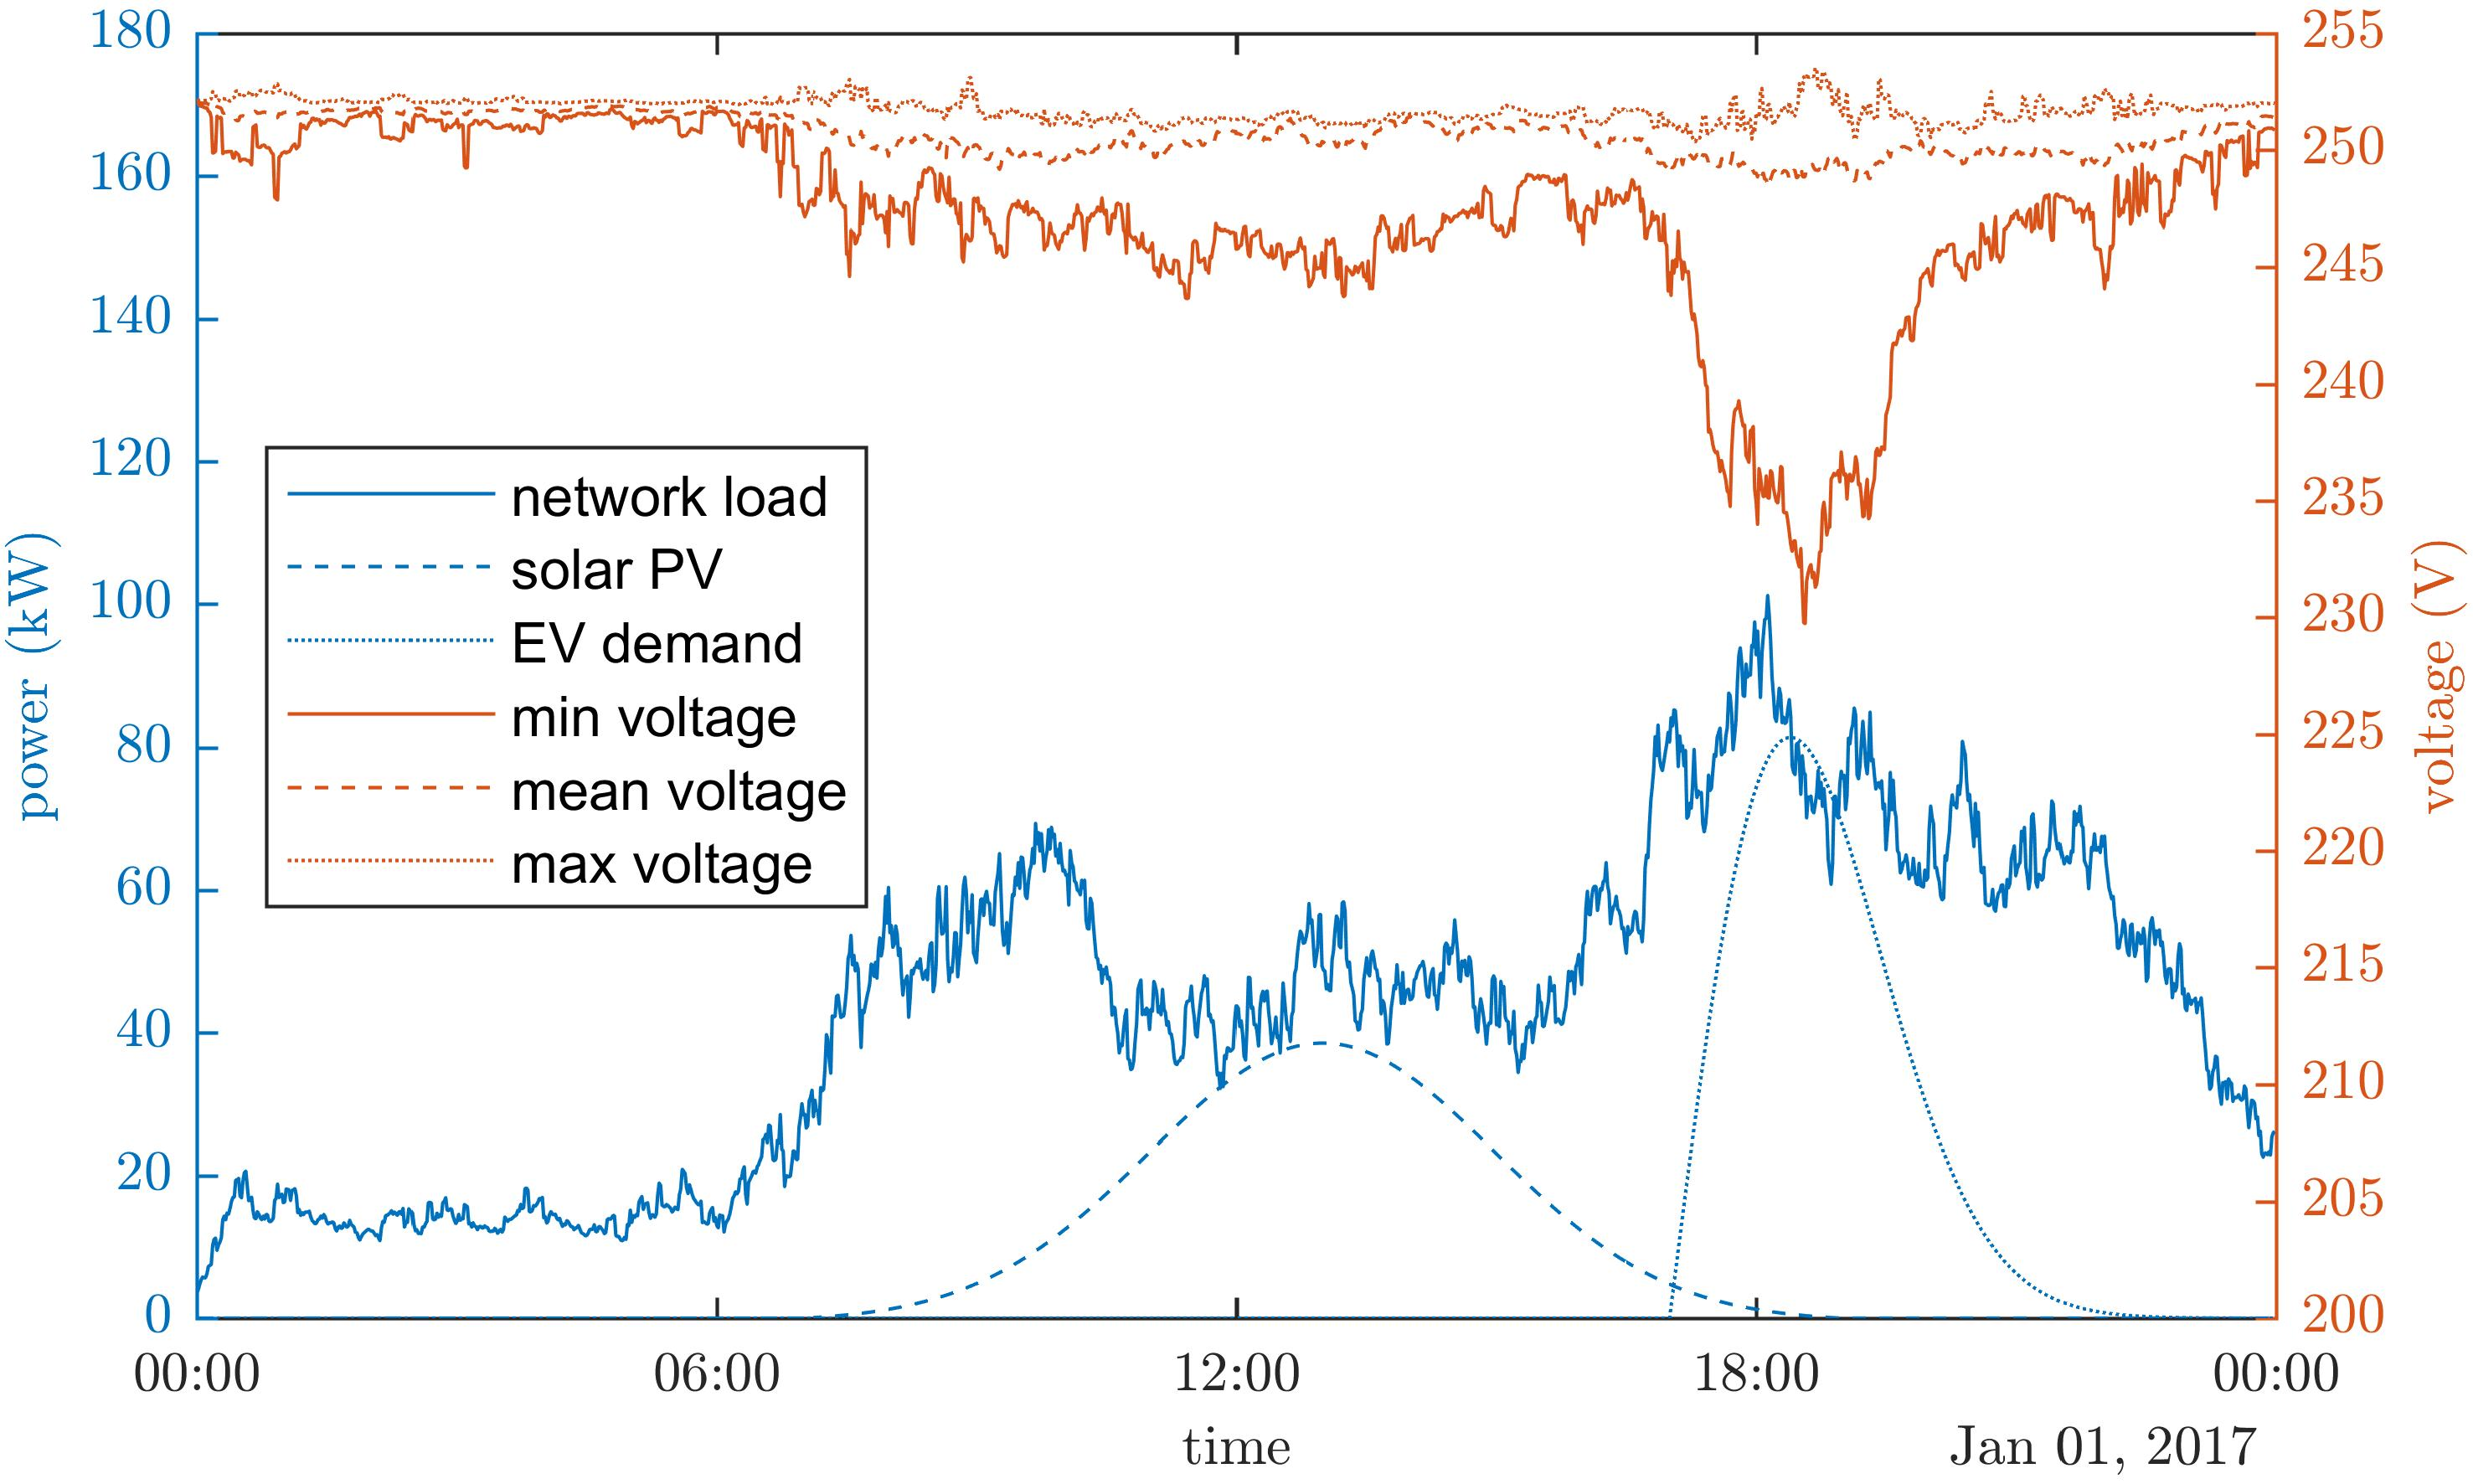
\includegraphics{_introduction/fig/lct-impact-with}
		\label{ch-introduction:subfig:lct-impact-with}
	}
	\caption{Study that compares impact on network voltages due to an uptake in LTCs on the IEEE LV test case: (a) does not contain any PV generation or EV loads; in (b) 20\% of all customers have PV generation with a peak generation of 3.5kW \cite{MongooseEnergy2015} and 20\% of all customers own EVs with Mode-2 home-charging capabilities at 7.4kW \cite{SustainableEnergyAuthorityofIreland2015}.}
	\label{ch-introduction:fig:lct-impact}
\end{figure}

Such a voltage drop behaviour was achieved with a relatively low rate of LCT adaptation in the residential environment, therefore strict regulation is in place to assure continuous operation without violating any operating constraints.
Otherwise additional voltage deviation, unbalanced network operation or potential asset overloads could be the result.

Traditional network planning approaches to follow these regulation were used to circumvent constraint violations.
These approaches follow the commonly used practice of aggregating a large number of customers and designing the power delivery network to cater for their largest probable demand, i.e. the After Diversity Maximum Demand (ADMD) method \cite{Richardson2010a}.
This ADMD method has remained the same for many years and uses historical load analysis and standard growth assumptions that are both no longer valid in this unprecedented LCT uptake scenario \cite{Yunusov2016}.
To make things worse, LV networks in the UK are generally unmonitored once installed.
Distribution Network Operators (DNOs) have become aware of this issue and are developing updated planning strategies involving ``smart'' and ``flexible'' electricity grids \cite{Fang2012}.
However, in situ equipment that will become subject to the same adaptation of LCT needs to be managed actively via innovation in the use of existing and new technologies; otherwise both frequency of service disruptions and customer minutes lost will increase alongside the proliferation of LCTs \cite{Ault2008a}.

\subsection{Solutions to mitigate impact of LCT}
\label{ch-introduction:subsec:solutions-to-mitigate-impact-of-lct}

Two solutions exist, allowing DNOs to support LV network's operation: 
\begin{enumerate*}
	\item reinforcement of in situ network assets;
	\item deployment of network support equipment.
\end{enumerate*}
Whilst network reinforcement would certainly address immediate issues of current network capacity constraints, this approach is also the more expensive and disruptive option.
More specifically, customer will need to deal with outages during periods of asset upgrades (e.g. transformer upgrade and line re-conductoring after secondary transformers' tap settings have been adjusted).
Therefore, alternatives to defer or avoid network reinforcements have been sought and assessed \cite{Harrison2007, Zangs2016a, VanderKlauw2016d, Greenwood2017}.
Most promising alternatives are to install flexible and controllable Distributed Energy Resources (DERs), or more specifically: Battery Energy Storage Solutions (BESS) \cite{Wade2010}.
BESS has not only seen significant advancements in technology, but also received increasing attention in both academic studies and industry trials \cite{Palizban2016}.

Installing BESS on a strategic location in the LV network brings several advantages to DNOs' control over the network's performance.
Roles for BESS are addressed in the subsequent section, i.e. Section \ref{ch-introduction:subsec:role-of-energy-storage-a-survey}.
However, a few examples of potential benefits from BESS include the regulation of voltages to stay within statutory operating bands \cite{Yang2014}, shaving peak loads to relieve stress from the installed network assets \cite{Bennett2015}, and reducing phase unbalance to increase network efficiency \cite{Wang2015b} .
Whilst the questions regarding locating and scaling of BESS have mostly been addressed, BESS control can be split into two complementing yet unmarried approaches:

\begin{enumerate}
	\item ``off-line'' control, using load forecasts and BESS schedules, and
	\item ``on-line'' control, using Set-Points Control (SPC), Model Predictive Control (MPC) or similar dynamic control methods.
\end{enumerate}

Furthermore, with the anticipated uptake of household BESS, mechanisms to control several storage systems also need to be considered.
For instance, several industry leaders propose to store solar energy in order to support charging of EVs \cite{Baumann2017}.
Without rooftop PV installations, batteries need work in a cooperative manner to not impose additional strain onto the network.
The full review of storage control strategies to achieve both off-line and on-line, as well as centralised/individual and distributed battery control is presented in Section \ref{ch-literature:sec:control-of-energy-storage}.

\subsection{Role of energy storage - a survey}
\label{ch-introduction:subsec:role-of-energy-storage-a-survey}


\begin{figure}\centering
	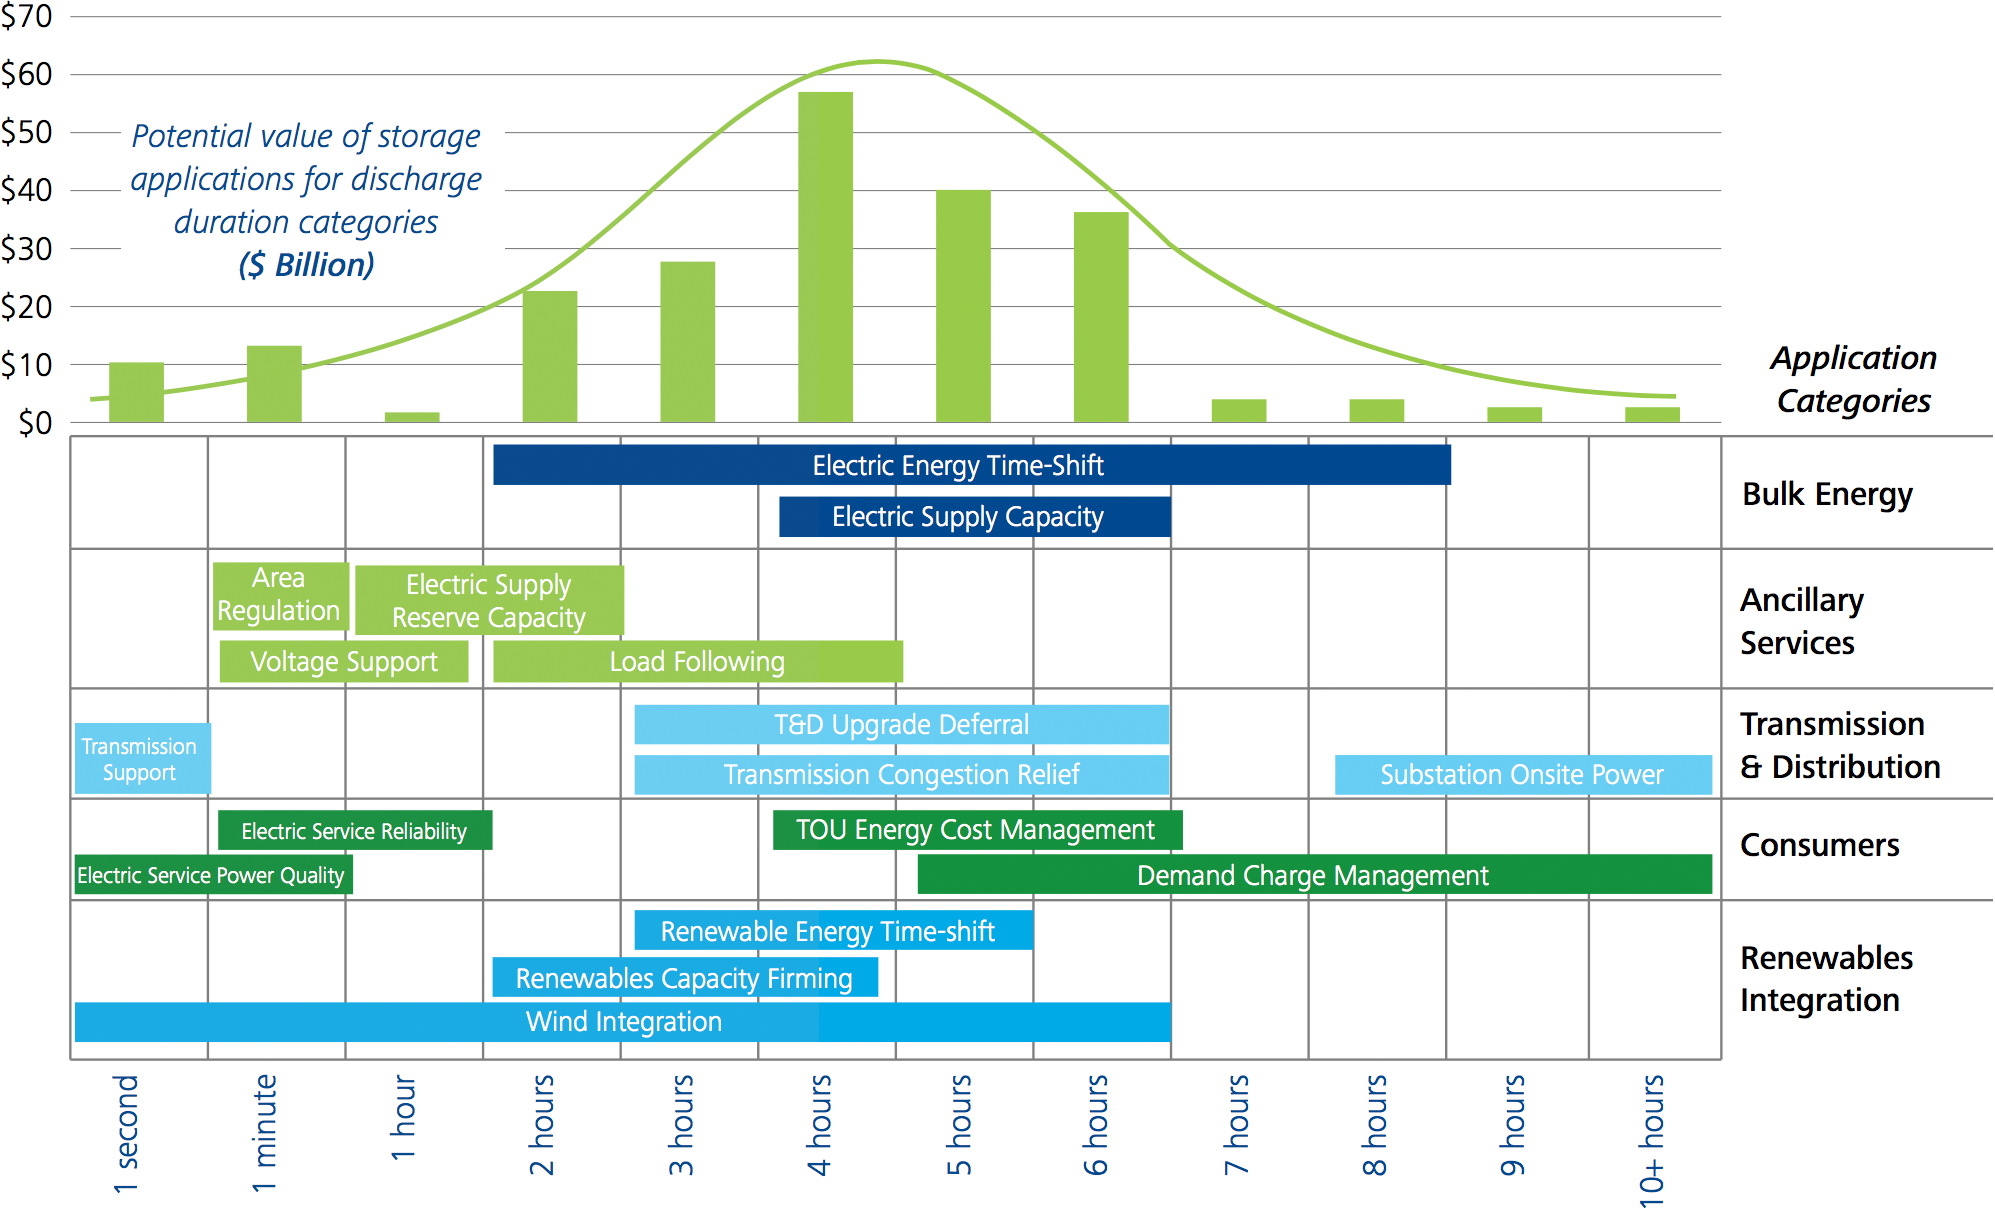
\includegraphics[width=\textwidth]{_introduction/fig/storage-financial-benefits}
	\caption{Energy storage applications and corresponding value for various discharge durations \cite{Deloitte2016}}
	\label{ch-introduction:fig:storage-financial-benefits}
\end{figure}

The idea of using energy storage in the electricity grid has been discussed for quite some time, and its important role in future energy systems has already been identified in the 70s \cite{Kalhammer1979}.
As the name suggests, electrical energy storage systems have the ability to both consume, store, and release electrical energy by converting it into a different form of energy.
Depending on the rate at which energy can be consumed and released, i.e. the system's power, as well as the amount of energy that can be stored, i.e. system's capacity, different functions can be provided.
A study for the Department Of Energy (DOE) showed that, when correctly exploited, these functions can yield direct financial benefits of \$157.56 billion over an estimated 10 year system lifecycle \cite{Eyer2010a}.
Figure \ref{ch-introduction:fig:storage-financial-benefits} shows these benefits in relation to their typical discharge period, and links them to their associated functions, too.
Here, Time Of Use (TOU) energy cost management yields the largest economic profit, yet from a historical point of view, bulk energy storage has played the most important role in the energy system.

Nowadays, storage can also tap into emerging revenue streams and perform additional functions.
As identified in several review articles \cite{Chen2009, Katsanevakis2017, Guney2017}, the key roles and applications of energy storage systems, regardless of profitability in the current market situation, can be identified as follows:

\textbf{Energy shifting - arbitrage}: This function uses the difference in energy price to yield revenue.
More specifically, as energy pricing is expected to become more dynamic and responsive to current energy demand and generation, storage is controlled to charge when energy prices are low and discharge when energy prices are high \cite{Chen2009, Leou2012}.
Such dynamic pricing schemes are expected to emerge due to significant changes in demand at morning and evening peaks \cite{Koohi-Kamali2013}.

\textbf{Supply capacity}: In order to meet future energy demand, energy suppliers commit their resources in advance.
Doing so allows them to plan for their operation and solve the economic dispatch problem.
With increasing demand, the supply volume will have to increase, too.
However, it is predicted that energy storage can defer or even avoid investments in power plants, assuming they are sized accrodingly (i.e. several 100MW)\cite{Dobie1998}.
Bulk energy storage was the first choice to support supply capacity.
One example is pumped hydro-electric energy storage, which has seen a global growth of 127GW since 1979 \cite{Rehman2015, Barbour2015, Barbour2016}.

\textbf{Ancillary services}: These services are of interest to transmission and distribution system operators since they support the operation of their networks.
For example, load following and frequency regulation are two complementing applications of that address the imbalance between demand and supply \cite{Bevrani2011}.
In case of a severe imbalance that resulted in network outage, black start is also a function that can be supplied by energy storage \cite{Cole1995, Kashem2007}.
Since modern energy storage systems can absorb and inject both active and reactive power, they can also provide voltage support \cite{Kulkarni2005}.

\textbf{Grid stability}: To make the grid more resilient to network faults (e.g. short-circuit or loss of a large generator), or to overcome scheduled network outages, energy storage can be used as an intermittent energy source \cite{Kundur1993}.
To provide optimal operation conditions for energy generators, storage can support rotor angle stability and voltage stability by injecting active and reactive power at the point of common coupling \cite{Chakraborty2012, Kolluri2002}.
Furthermore, sub-synchronous resonance and harmonic interference can also be reduced \cite{Wang1994}.
This coupling resonance can occur between electrical and mechanical systems and can damage the mechanical structure due to repetitive stresses and strains.

\textbf{Upgrade deferral}: As already stated in Section \ref{ch-introduction:subsec:solutions-to-mitigate-impact-of-lct}, both transmission and distribution systems would have to be upgraded unless energy storage could provide network-support functions.
By deferring network upgrades, network assets will be used more efficiently, and customer disruptions will be avoided \cite{Sayer2007, Eyer2010a}.
Furthermore, in areas where the expected load has already been met and growth has levelled out, deployed energy storage is flexible enough to provide alternative functions (unlike other network assets) \cite{Huff2013}.

\textbf{Transmission charges}: In scenarios where generators are charged to use transmission systems (due to the capacity limitations of the transmission system), energy storage could take advantage of the price structure to maximise the profit from the generated energy \cite{Sayer2007, Leou2012}.

\textbf{Congestion relief}: High congestion at substations of heavily loaded transmission or distribution lines can be tackled by co-located energy storage units \cite{Saez-de-Ibarra2013a, Kulkarni2005}.
This can be achieved by e.g. shaving peak load or relaxing the energy requirements from distributed generation \cite{Reihani2016, Gerards2016d}.

\textbf{Service reliability}: In areas where a string grid connection is required to assure e.g. industry operations, an ``uninterruptible power supply'' may be required.
Traditionally, these power supplies were diesel backup generators, but modern energy storage technology can provide similar services at lower cost \cite{Schoenung2001} (particularly when including alternative revenue streams).

\textbf{Power quality}: Sub-cycle and harmonic distortions on can severely deteriorate power quality, since they can have unwanted effects on connected equipment (similar to the issue of sub-synchronous resonance at the generation side).
Energy storage with modern power electronics could be capable of providing power filtering functions that suppress those distortion \cite{Putrus2007}.
This feature could be of particular interest to LV networks in the UK, since customers are arbitrarily connected to a single phase of a three-phase network.
Therefore, the discrepancy of power quality between the phases is even larger, yet available energy storage resources could even address this issue \cite{Miret2009} (especially when considering household connected units).


\textbf{Time-of-use energy charges}: A hurdle to DSM through flexible tariffs or TOU tariffs is the reason that consumers would have to adjust their energy consumption based on external price signals, which many are do not want to do.
Energy storage could however decouple the consumer form these tariffs and allow them to continue with their normal lifestyle \cite{Khani2014}.
Additionally, when exploiting the energy price difference, storage could even supply arbitrage functions to some customers and reduce their electricity bill \cite{Nair2010a}.
For customers with local generation, e.g. PV installation, their bill can be reduction even further.
This would be done by storing the generated energy until a period of high energy prices arises.
At this time energy storage could release the energy to maximise self-consumption \cite{Luthander2016}.

\textbf{Demand charges}: Larger customers, i.e. industrial and commercial loads, are not only charged for their total energy demand, but also their for their largest continuous power demand \cite{Oudalov2007, Mackey2013}.
Therefore, a factory that may use a relatively small amount of energy over a comparatively short amount of time, is billed accordingly.
After all, the infrastructure to deliver the required power needs to be installed and maintained.
In this scenario, energy storage could reduce the intermittent power demand without significantly increasing the total energy demand, and therefore reduce demand charges for larger customers \cite{Aghaei2013}.

\textbf{Renewables integration}: Unlike traditional energy sources, renewables have are highly volatile and have limited availability.
Since their availability, i.e. for solar PV, may not align with periods of high demand, i.e. during morning and evening, arbitrage functions may be provided to maximise the use of renewable generation - i.e. renewables ``shifting'' \cite{Zakeri2015}.
Furthermore, by discharging energy storage during times of low renewable generation, e.g. due to cloud cover or varying wind \cite{Jewell1987}, a continuous supply of energy can be assured - i.e. renewables ``smoothing''.
And lastly, if a renewable resource was committed for longer periods of time, yet the associated energy forecasts overestimated its generation capacity, storage can supply the gap to avoid balancing charges - i.e. renewables ``firming'' \cite{Chakraborty2012}.

\subsection{Smart control}
\label{ch-introduction:subsec:smart-control}

\hl{WRITE THIS}

\subsection{Challenges to control BESS}
\label{ch-introduction:subsec:motivation}

From the extensive catalogue of possible roles for energy storage in the electricity grid that was presented in Section \ref{ch-introduction:subsec:role-of-energy-storage-a-survey}, the focus of the research in this thesis is put on aiding DNOs to manage and operate their power distribution networks.
More specifically, battery energy storage is the main focus since is has the potential to defer or even mitigate costly network reinforcements.
Modern battery technology allows the storage of electrical energy in ever-decreasing form factory, whilst power electronics technology becomes more efficient at integrating batteries into power networks.

As shown in the literature review in Chapter \ref{ch-literature}, methods of controlling BESS to optimise power flow have been of great research interest.
However, the impact on particular key parameters of the three-phase networks still need to be investigated.
Subsequently, the challenge of applying real-time corrections to BESS schedules in order to decrease peak demand whilst obeying to technical and operational constraints is also a remaining research question.
Also, since the expected uptake of distributed BESS through proliferation of household storage solutions (e.g. to counteract the impact of EVs) requires sophisticated coordination mechanisms, two additional research challenges have been identified.
The first challenge focuses on improving cooperating device behaviour despite communication disturbances (i.e. through message desynchronisation), and the second builds upon the findings from key network improvements to construct a functioning BESS control mechanism despite the absence of a telecommunications infrastructure.







\section{Problem statement and research objectives}
\label{ch-introduction:sec:problem-statement}

The focus of the research presented in this thesis is put on aiding DNOs to manage and operate their power distribution networks by installing energy storage into their distribution networks in order to counteract the effects from electrification of heat and transport sectors as well as the decarbonisation of the grid itself.
Therefore BESS control is the main focus of this work since BESS is a rapidly improving technology that has the potential to defer or even mitigate costly network reinforcements.
Modern battery technology allows the storage of electrical energy in ever-decreasing form factors, whilst power electronics technology becomes more efficient at integrating batteries into power networks.
As shown in the literature review in Chapter~\ref{ch-literature}, methods to control BESS, for instance, in order to optimise power flow, have been and still are of great research interest.

Therefore, the aim of this thesis is to present a contribution in BESS control to improve grid operation and reliance, when deploying it in the UK LV distribution network.
Given the already established control approaches of ``off-line'' and ``on-line'' control, merging the two in order to take advantage of BESS schedules and real-time information is still an open research challenge.
Subsequently, applying real-time corrections to BESS schedules in order to decrease peak demand whilst obeying to technical and operational constraints is also an identified research challenge.
Since the expected uptake of distributed LCTs and DERs through proliferation of household-connected storage solutions (for example to support PV integration or to counteract EV impacts) requires ``smart'' coordination mechanisms.
When requiring communication to implement this smart coordination, another challenge exists in developing algorithms that function despite communication disturbances (i.e. through message desynchronisation).
Lastly, in the case where communication-less coordination of distributed devices is sought, the challenge of assuring equal device usage whilst providing network support (for example to guarantee a minimum lifetime) has also been identified.

These research challenges are extensively reviewed in the literature review in Chapter \ref{ch-literature}, and in accordance to these identified key challenges that motivate the conducted research, a set of objectives is presented in order to achieve the aim of contributing to the existing field:

\begin{enumerate}[
labelindent=*,
style=multiline,
leftmargin=*,
label=\textbf{Objective~\arabic*}
]
	\item \label{objective-1} Develop a control mechanism for a single BESS to further improve three-phase network operation without \hl{changing half-hourly real power schedules by adjusting BESS power phasors and reactive power injection}.
	\item \label{objective-2} Develop a control mechanism that \hl{dynamically adjusts half-hourly schedules on a sub-half-hourly basis, hence modifying the half-hourly schedule to reduce daily load peaks by combining control elements from both off-line and on-line control}.
	\item \label{objective-3} Develop and compare operation of a scheduling algorithm that manages the charging behaviour of multiple BESS by submitting it to performance analysis in a synchronised and desynchronised communication environment.
	\item \label{objective-4} Develop a communication less control strategy for distributed BESS by \hl{modifying the traditional and robust Additive Increase Multiplicative Decrease (AIMD) algorithm by introducing a threshold dependent scaling of the additive term} and by individually assigning control parameters.
\end{enumerate}



\section{Contributions to knowledge}
\label{ch-introduction:sec:contributions}

The literature that is reviewed in Chapter~\ref{ch-literature} introduces the key contributions surrounding the control of energy storage in power distribution networks, and therefore supports the thesis problem statement in Section~\ref{ch-introduction:sec:problem-statement}.
This review concludes by identifying gaps in literature which are used as starting points to formulate the research objectives and resulting research contributions.
These contributions are summarised as follows:

\begin{itemize}
	\item
	An iterative closed-loop power adjustment method is presented, which controls a DNO owned storage devices in such a way that its three-phase power flow improves LV network operation.
	This contribution is the result of \ref{objective-1} and is achieved by using the device's flexibility in assigning active power to the three phases, and by using the remaining capacity of power electronics to inject or absorb reactive power, whilst obeying to an underlying half-hourly BESS schedule.
	\item
	A dynamic control method to merge off-line BESS scheduled control with an on-line power prediction mechanism (i.e. Model Predictive Control) is developed to minimises both the imminent sub-half-hourly load peaks as well as the day-ahead half-hourly load peaks.
	This contribution is the result of \ref{objective-2} and is achieved by merging schedules that are based on real load forecasts with an autoregressive model that is fed by real load data.
	\item
	A robust charge scheduling algorithm for multiple, distributed entities is developed to prevent charging spikes from adding excessive stress onto the distribution network which would otherwise experience capacity shortages.
	This contribution is the result of \ref{objective-3} and is achieved by implementing a ``Multi-Agent System'' (discussed in the literature review in Section~\ref{ch-literature:subsec:centralised-and-distributed-control}) on a compute cluster to compare algorithm performance for both synchronised and desynchronised message exchange.
	\item
	A communication-less distributed control method is developed that improves the traditional Additive-Increase Multiplicative-Decrease (AIMD) algorithm to achieve cooperative behaviour of multiple BESSs in order to mitigate the impact of co-located ``dumb-charging'' EVs.
	This contribution is the result of \ref{objective-4} and is achieved by individually assigning control parameters to all BESS whilst using local voltage measurements to infer the current network status.
\end{itemize}


\section{Publications}
\label{ch-introduction:sec:publications}

%Throughout the course of the research that is presented in this thesis, results and outcomes have been disseminated and through the following publications:
%In addition to the first-authored publications, co-authored publications include:

\begin{itemize}

\item \textbf{First-authored publications:}
\begin{itemize}
	\item M. J. Zangs, P. B. E. Adams, T. Yunusov, W. Holderbaum, and B. A. Potter, ``Distributed energy storage control for dynamic load impact mitigation,'' Energies, vol. 9, no. 8, 2016.
	\item M. J. Zangs, T. Yunusov, W. Holderbaum, and B. Potter, ``On-line adjustment of battery schedules for supporting LV distribution network operation,'' in 2016 International Energy and Sustainability Conference, IESC 2016, 2016.
	\item M. J. Zangs, T. Yunusov, W. Holderbaum, and B. Potter, ``Battery control algorithm for peak load shaving in low-voltage power network with high demand volatility,'' Applied Energy (in review)
\end{itemize}

\item \textbf{Co-authored publications:}
\begin{itemize}
	\item T. Yunusov, M. J. Zangs, and W. Holderbaum, ``Control of Energy Storage,'' Energies, vol. 10, no. 7, p. 1010, 2017.
	\item T. Yunusov, M. J. Zangs, and W. Holderbaum, ``Online Control Algorithm for Sub-Half-Hourly Operation of LV-Connected Energy Storage Devices Owned by DNO'', in 24th International Conference \& Exhibition on Electricity Distribution (CIRED), CIRED 2017, 2017
\end{itemize}

\end{itemize}






\section{Thesis structure}
\label{ch-introduction:sec:thesis-structure}

The structure of this thesis is organised as follows:

\begin{itemize}
	\item
	\textbf{Chapter~\ref{ch-literature}} carries out an extensive review of the literature surrounding the field in order to support the problem statement and proposed contribution.
	\item
	\textbf{Chapter~\ref{ch1}} develops a BESS scheduling mechanism and identifies key network parameters that are used in their corresponding cost functions to improve network operation.
	Then, this chapter address \ref{objective-1} by presenting a method that assigns a BESS schedule to the three-phase power distribution network whilst minimising the aforementioned cost functions; therefore improving network operation.
	Results are compared against a ``baseline'' and a ``normal'' (or traditional) operation case by assessing them on a temporal and probabilistic level.
	\item
	\textbf{Chapter~\ref{ch2}} then extends the work in Chapter~\ref{ch1} by presenting a dynamic control method that adjusts a half-hourly BESS schedule at sub-half-hourly temporal resolution in order to reduce both volatile and the daily load peak.
	This is achieved by combining two PID compensated control loops with a MPC and BESS schedule.
	Therefore, this chapter addresses \ref{objective-2}.
	\item
	\textbf{Chapter~\ref{ch3}} addresses \ref{objective-3} by presenting a cooperative battery charging algorithm that is deployed on a Multi-Agent System and assessed in both a synchronised and desynchronised communication environment.
	In this chapter, both algorithm convergence and algorithm performance is compared between its implementation in the synchronised and desynchronised scenario.
	\item
	\textbf{Chapter~\ref{ch4}} develops a stochastic EV demand model that is based on real vehicle mobility data, and it will develop a control algorithm for distributed BESS to mitigate the negative impact from the resulting EV demand.
	This chapter address \ref{objective-4}, the final research objective, by extending the Additive-Increase Multiplicative-Decrease algorithm to enable cooperating BESS operation under the absence of a shared communication infrastructure.
	\item
	\textbf{Chapter~\ref{ch-conclusions}} presents a detailed conclusion that relates all findings back to the initial problem statement and the overarching aim of the presented PhD thesis.
	Also, this chapter highlights potential future work based on the findings from the conducted research.
\end{itemize}